\documentclass{article}

\usepackage[dutch]{babel}
\usepackage[margin=3cm]{geometry}
\usepackage{graphicx}
\usepackage{float}
\usepackage{caption}
\usepackage{hyperref}
\usepackage{amsmath}
\usepackage{wrapfig}


\graphicspath{{img/}} 
 
\newcommand{\bold}[1]{\textbf{#1}}
 
\begin{document}

\begin{titlepage}
    \author{Tuur Vanhoutte}
    \title{Sensors \& Interfacing}
\end{titlepage}

\pagenumbering{gobble}
\maketitle
\newpage
\tableofcontents
\newpage

\pagenumbering{arabic}

\section {Communicatie}
\subsection{Datacommunicatie in IoT}
\subsubsection{De 3 lagen}
\begin{enumerate}
    \item Application Layer
    \item Fog layer
    \item IoT Device Layer
\end{enumerate}


\begin{figure}[H]
    \centering
    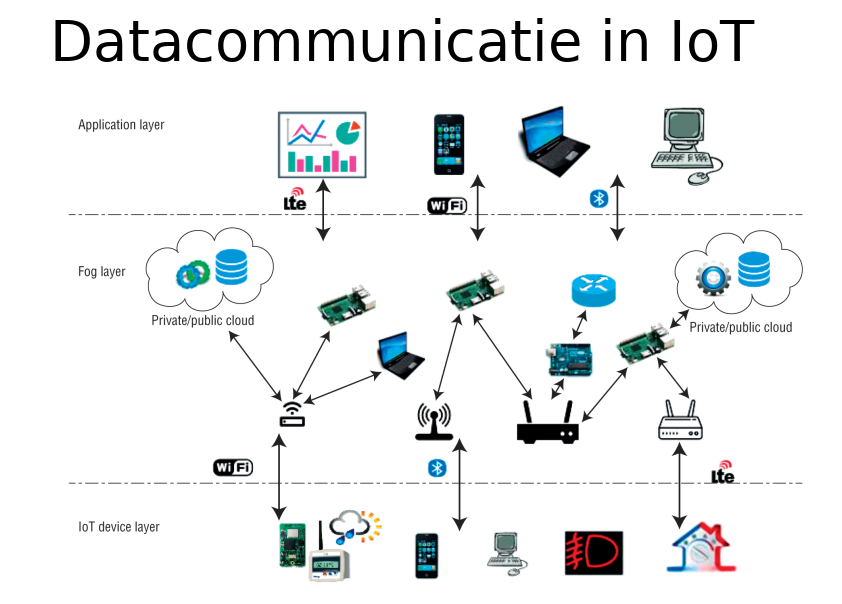
\includegraphics[width=0.95\textwidth]{Screenshot_20200210_120010.png}
    \caption{Datacommunicatie in IoT}
\end{figure}



\subsection{Data}
\begin{itemize}
    \item "Pre-informatie"
    \item Gegevens waaruit informatie kan worden gewonnen
    \item Stelt een bepaalde toestand voor
    \item \url{https://en.wikipedia.org/wiki/Data}
\end{itemize}

\subsection{Communicatie}
= Overbrengen van informatie tussen deelnemers
\begin{itemize}
    \item Boodschap
    \item Signaal
    \item Medium
\end{itemize}

\subsection{Communicatieafspraken}
\begin{itemize}
    \item Coderen van informatie (encoding)
    \item Voorbeelden:
    \begin{itemize}
        \item morse-code
        \item Ascii-codering
        \begin{itemize}
            \item Codering voor alle gebruikte symbolen in symbolen
            \item Codering in 7 of 8 bit
            \item 1 byte = 1 teken
        \end{itemize}
        \item \dots
    \end{itemize}
\end{itemize}
  
\subsection{Encoding/Decoding}
3 stappen:
\begin{enumerate}
    \item Codifying
    \item Sending the message
    \item Decodifying
\end{enumerate}

\subsection{Signalen}
\begin{itemize}
    \item Licht
    \item Geluid
    \item Elektriciteit
    \item \dots
\end{itemize}

\subsection{Communicatiemedia}
\begin{itemize}
    \item Twisted-Pair cable
    \item Coaxial cable
    \item Fiber-Optic cable
\end{itemize}

\begin{figure}[H]
    \centering
    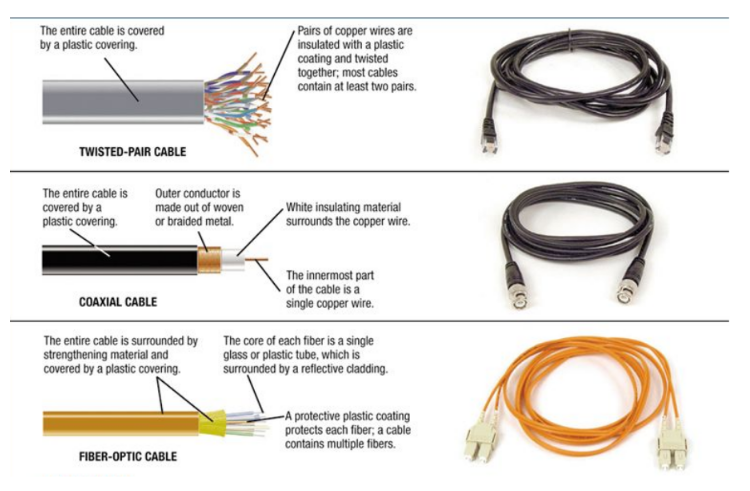
\includegraphics[width=\textwidth]{Screenshot_20200315_105647.png}
    \caption{Soorten kabels}
\end{figure}


\subsubsection{Eigenschappen van media}
\begin{itemize}
    \item Vatbaarheid voor interferentie
    \item Overbrugbare afstand
    \item Praktisch
    \item Kostprijs
    \item \dots
\end{itemize}

\subsubsection{Afspraken}
\begin{itemize}
    \item Protocol
    \item Standaarden
    \item IEEE
    \item EIA (NEDA/ECA) $\Rightarrow$ ECIA
\end{itemize}

\subsubsection{Standaardiseren van \dots}
\begin{itemize}
    \item Type media en zijn specificaties
    \item Het gebruikte signaal en zijn toleranties
    \item De elektrische interferentie
    \item De gebruikte codering
    \item Foutcorrectiecodes
    \item Protocol
    \item De gebruikte connector
    \item \dots
\end{itemize}

\section{Analoog vs digitaal}
\begin{itemize}
    \item \bold{Digitaal}: Discrete waarden
    \item \bold{Analoog}: Continue waarden
\end{itemize}
\subsection{Toestanden}
\subsubsection{Bepaalde toestand}
\begin{itemize}
    \item Temperatuur
    \item Licht aan/uit
    \item Afstand
    \item Tijd
    \item \dots
\end{itemize}

\subsubsection{Digitale toestanden}
\begin{itemize}
    \item Licht aan/uit
    \item Deur open/dicht
    \item Keuze van versnelling N - 1 - 2 - 3 - 4 - 5 - R
    \item Ruitenwisser interval uit - interval - traag - snel
    \item \dots
\end{itemize}

\subsubsection{Analoge toestanden}
\begin{itemize}
    \item Tijd (!)
    \item Temperatuur
    \item Luchtdruk
    \item Luchtvochtigheid
    \item Afstand
    \item \dots
\end{itemize}


\subsection{Signalen}
\begin{itemize}
    \item Analoog signaal
    \item Digitaal signaal
\end{itemize}

\begin{figure}[H]
    \centering
    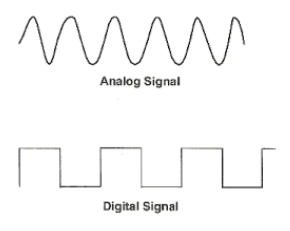
\includegraphics[width=0.4\textwidth]{Screenshot_20200217_115642.png}
    \caption{Analoog vs digitaal signaal}
\end{figure}
\section{Analoge signalen}

\subsection{Omzetten van analoge signalen}

\subsubsection{Transducer}
Omzetten van een analoog signaal naar een ander analoog signaal.\\
\bold{Voorbeeld}: elektrisch signaal omzetten naar een geluidsignaal via een luidspreker (=de transducer)

\begin{figure}[H]
    \centering
    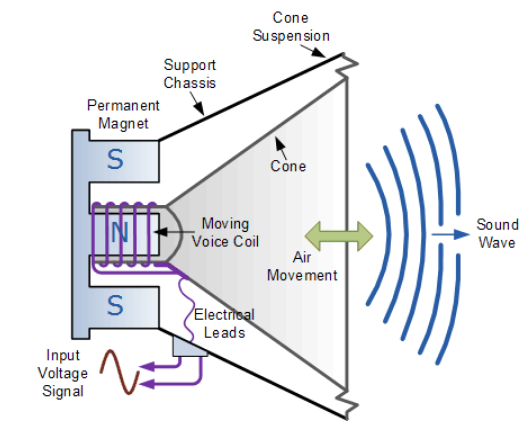
\includegraphics[width=0.4\textwidth]{Screenshot_20200315_111132.png}
    \caption{Luidspreker}
\end{figure}

\subsubsection{Sensoren en Actuatoren}
\begin{itemize}
    \item Sensor $\Rightarrow$ meten van een fysieke eigenschap
    \item Actuator $\Rightarrow$ be"invloeden van een fysieke parameter $\Rightarrow$ transducers 
\end{itemize}

\subsection{Analoge communicatie}

\begin{figure}[H]
    \centering
    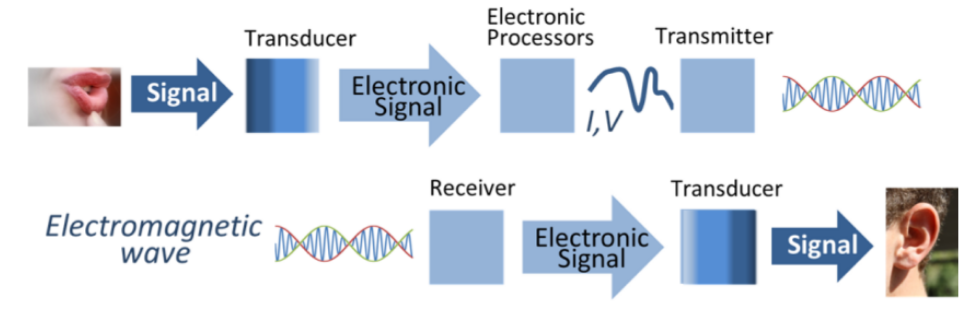
\includegraphics[width=0.5\textwidth]{Screenshot_20200315_111720.png}
    \caption{Analoge communicatie}
\end{figure}

\subsection{Analoog signaal}
Sinusgolf als meest elementaire signaal

\begin{figure}[H]
    \centering
    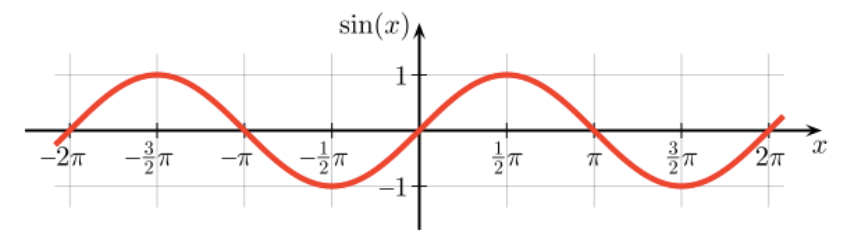
\includegraphics[width=0.5\textwidth]{Screenshot_20200315_113310.png}
    \caption{Sinusgolf}
\end{figure}

\subsubsection{Eigenschappen}
\begin{itemize}
    \item DC vs AC
    \item Polariteit blijft gelijk bij (pulserende) DC
    \item Polariteit verandert bij AC
\end{itemize}



\begin{figure}[H]
    \centering
    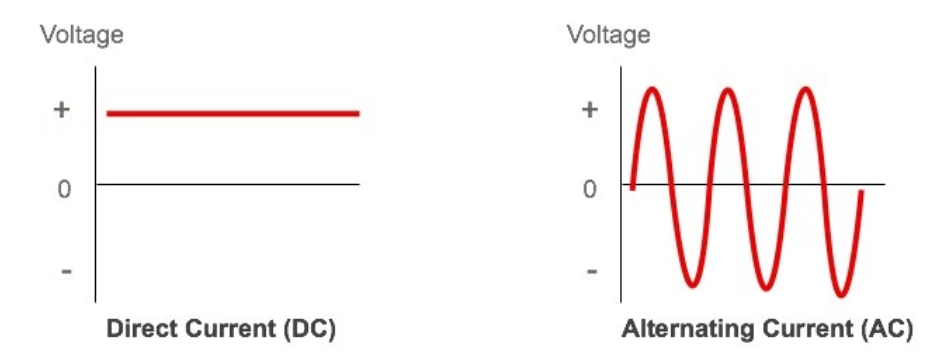
\includegraphics[width=0.5\textwidth]{Screenshot_20200217_121011.png}
    \caption{DC vs AC}
\end{figure}

\subsubsection{Wisselspanning - Eigenschappen}
\begin{itemize}
    \item RMS = Root Mean Square (= kwadratisch gemiddelde) = effectieve waarde (in geval van sinus)
    \begin{enumerate}
        \item Som van alle kwadraten (= square)
        \item Die som delen door het aantal waardes (= mean)
        \item Neem de vierkantswortel van dat getal
    \end{enumerate}
    \begin{itemize}
        \item Wordt vaak gebruikt in de elektriciteit om het gemiddelde vermogen te vinden
    \end{itemize}
    \item Frequentie
    \item Periode
    \item Amplitude
    \item Peak of top-to-top waarde
\end{itemize}

\begin{figure}[H]
    \centering
    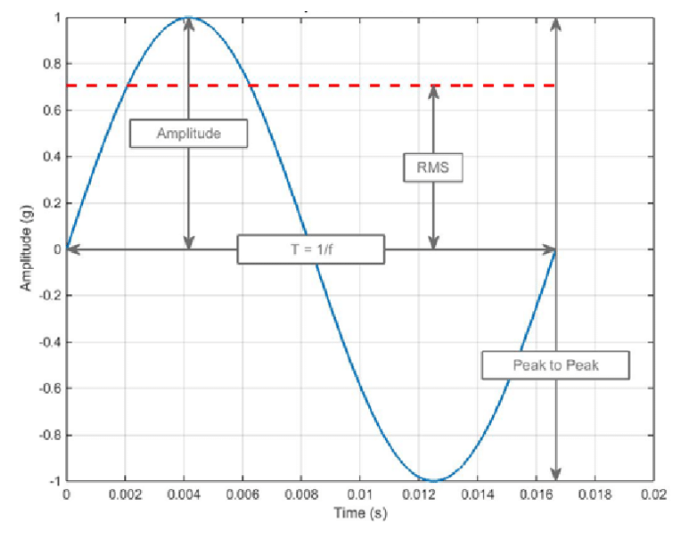
\includegraphics[width=0.7\textwidth]{Screenshot_20200217_121136.png}
    \caption{Eigenschappen wisselspanning}
\end{figure}

\subsubsection{Periodieke signalen}
\begin{itemize}
    \item 1 herhaling = 1 periode
    \item Periode (T) = tijdsduur (in s)
    \item Frequentie (f) = aantal periodes per seconde (in Hz)
    \item $F = \frac1T$ $\Leftrightarrow$ $T = \frac1F$
\end{itemize}

\begin{figure}[H]
    \centering
    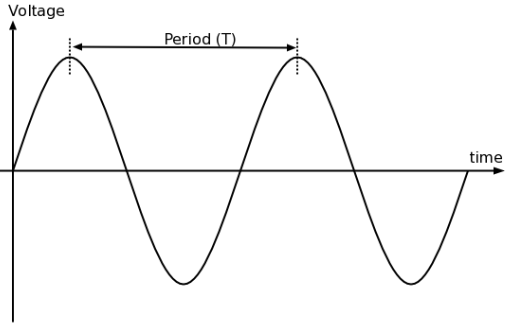
\includegraphics[width=0.4\textwidth]{Screenshot_20200217_122002.png}
    \caption{Sinusgolf met periode $T$}
\end{figure}


\subsubsection{Tijdsdomein en frequentiedomein}
\begin{itemize}
    \item Tijdsdomein: met een oscilloscoop
    \item Frequentiedomein: met spectraalanalyse 
\end{itemize}

\begin{figure}[H]
    \centering
    \centerline{
        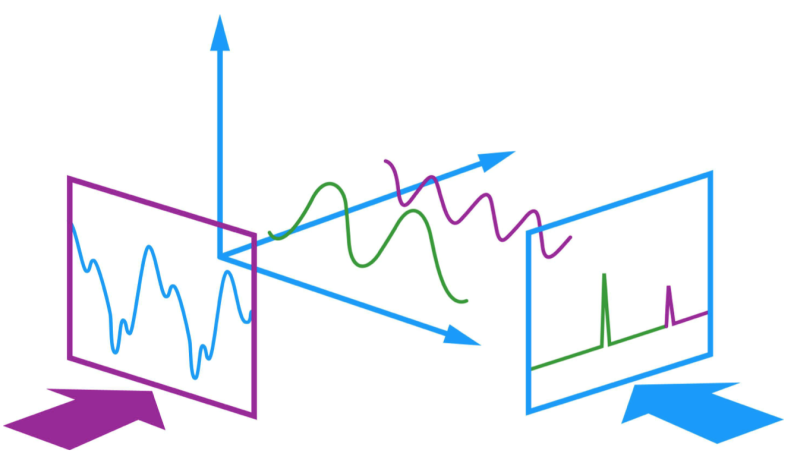
\includegraphics[width=0.4\textwidth]{Screenshot_20200217_122108.png}
        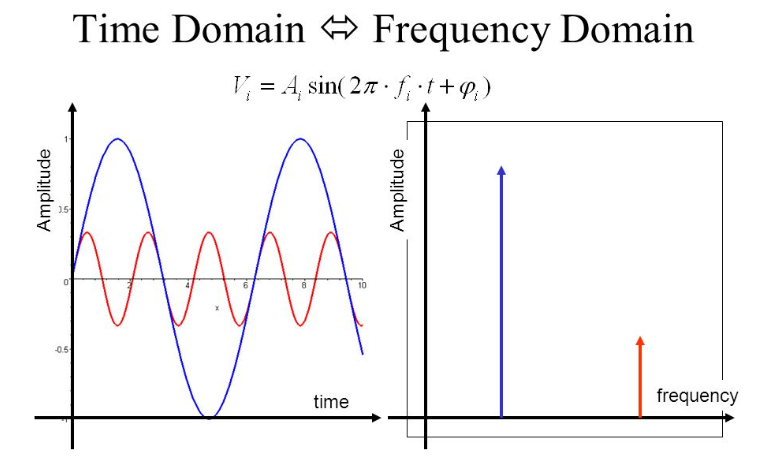
\includegraphics[width=0.5\textwidth]{Screenshot_20200217_122246.png}    
    }
    \caption{Tijdsdomein vs Frequentiedomein}
\end{figure}

\section{Digitale signalen}
= Aan/uit

\subsection{Eigenschappen}
\begin{itemize}
    \item Amplitude: Piek- of top-waarde, RMS-waarde
    \item Periode / frequentie
    \item Pulsbreedte 
    \item Duty-cycle
\end{itemize}


\begin{figure}[H]
    \centering
    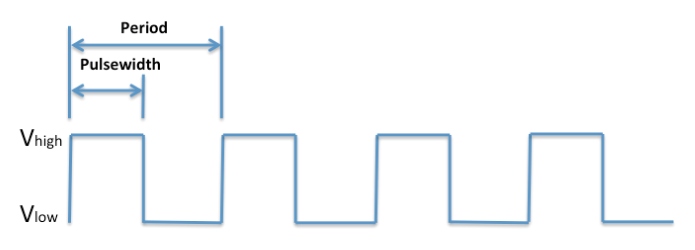
\includegraphics[width=0.9\textwidth]{Screenshot_20200315_120112.png}
    \caption{Eigenschappen digitaal signaal}
\end{figure}

\subsection{Duty Cycle}
= Hoeveel procent van de tijd staat het signaal aan?

\begin{figure}[H]
    \centering
    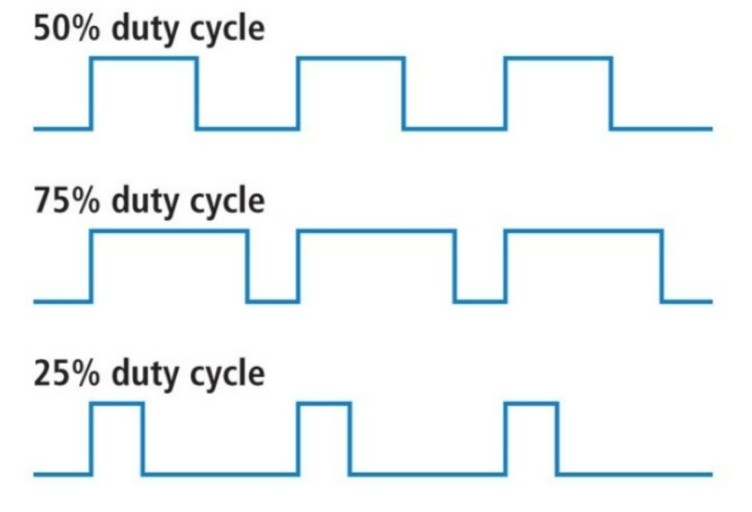
\includegraphics[width=0.5\textwidth]{Screenshot_20200315_120616.png}
    \caption{Duty cycles}
\end{figure}

\subsection{Flanken (edge)}
\begin{itemize}
    \item Stijgende flank
    \item Dalende flank
    \item Belangrijk bij kloksignalen
\end{itemize}

\begin{figure}[H]
    \centering
    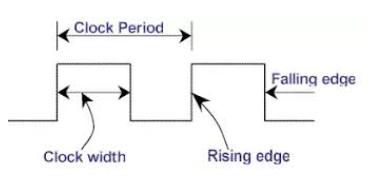
\includegraphics[width=0.5\textwidth]{Screenshot_20200217_123230.png}
    \caption{Flanken}
\end{figure}

\subsection{Weergave digitale signalen}

\begin{figure}[H]
    \centering
    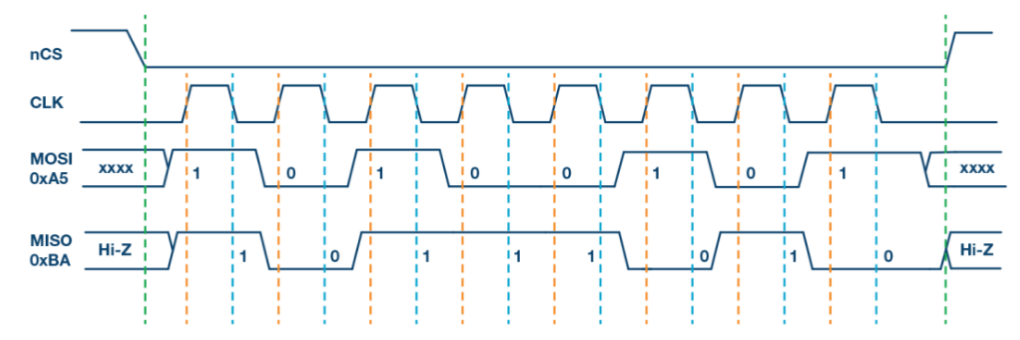
\includegraphics[width=0.8\textwidth]{Screenshot_20200217_125726.png}
    \caption{Weergave digitale signalen}
\end{figure}


\section{AD conversie}

\begin{figure}[H]
    \centering
    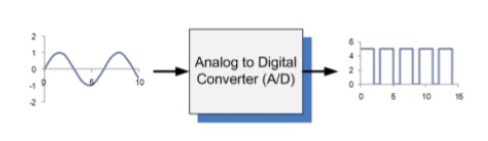
\includegraphics[width=0.7\textwidth]{Screenshot_20200224_115204.png}
    \caption{Analoog naar digitaal (AD converter)}
\end{figure}

\subsection{Analoog naar digitaal}

\begin{figure}[H]
    \centering
    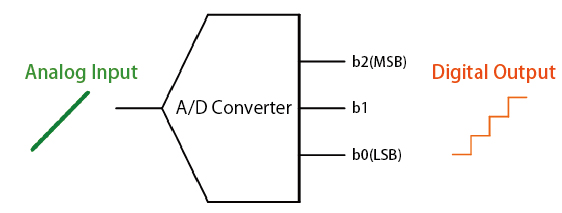
\includegraphics[width=0.7\textwidth]{Screenshot_20200224_115430.jpg}
    \caption{Analoog naar digitaal conversie}
\end{figure}

\begin{itemize}
    \item \bold{Range} = verschil tussen laagste en hoogste waarde
    \item \bold{Resolutie} = aantal stappen of stapgrootte in bits
    \item \bold{Belangrijk gevolg:}
    \begin{itemize}
        \item beide parameters bepalen de exactheid en de afwijkingen
    \end{itemize}
\end{itemize}

\subsubsection{Voorbeeld A}
\begin{itemize}
    \item Range = 2V - 2.5V
    \item Resolutie = 8bits
    \item Dus aantal discrete stappen = $2^8 = 256 \Rightarrow 256 - 1 = 255$
    \item Stapgrootte (LSB) = $\frac{range}{255} = \frac{2.5V - 2V}{255} = \frac{0.5V}{255} = 0.00196..V / stap$
    \item ofwel $\approx$ $2mV$/stap
\end{itemize}


\subsubsection{Voorbeeld B}
\begin{itemize}
    \item Range = 0V - 12V
    \item Resolutie = 12bits
    \item Dus aantal discrete stappen = $2^{12} = 4096 \Rightarrow 4096 - 1 = 4095$
    \item Stapgrootte (LSB) = $\frac{range}{4095} = \frac{12V - 0V}{4095} = \frac{12V}{4095} = 0.0029304..V / stap$
    \item ofwel $\approx$ $3mV$/stap
\end{itemize}

\subsection{Eigenschappen}

\subsubsection{Quantisatiefouten}

\begin{figure}[H]
    \centering
    \centerline{
        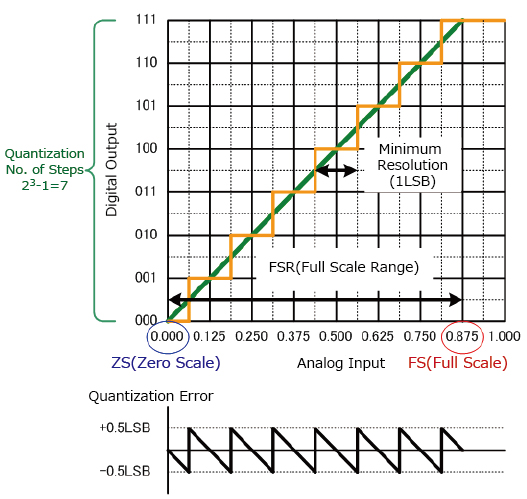
\includegraphics[width=0.5\textwidth]{Screenshot_20200224_120800.jpg}
        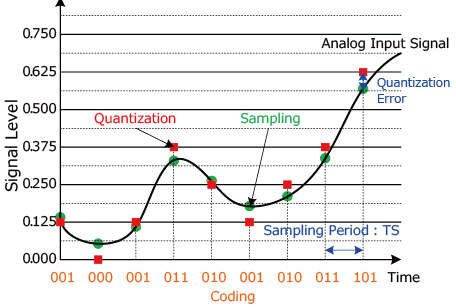
\includegraphics[width=0.5\textwidth]{Screenshot_20200224_120900.jpg}    
    }
    \caption{Quantisatiefouten door AD conversie}
\end{figure}

\begin{itemize}
    \item Verzorzaakt quantisatieruis
    \item Quantisatiefouten $\rightarrow$ dithering
    \item = \underline{vooraf} (witte) ruis toevoegen aan signaal
\end{itemize}

\begin{figure}[H]
    \centering
    \centerline{
        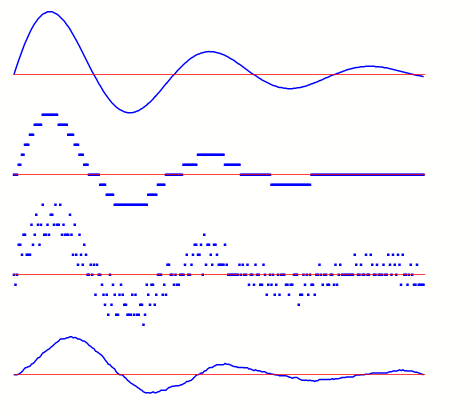
\includegraphics[width=0.4\textwidth]{Screenshot_20200224_121151.png}
        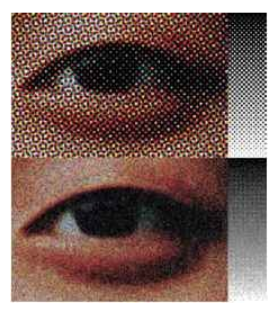
\includegraphics[width=0.3\textwidth]{Screenshot_20200315_122540.png}
    }
    \caption{Dithering}
\end{figure}

\subsubsection{Sample Rate / sample frequentie}
= aantal conversies per seconde
\begin{figure}[H]
    \centering
    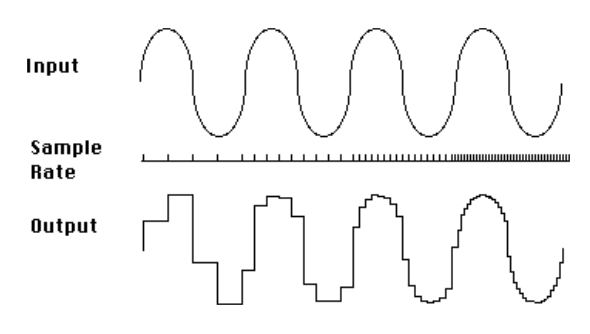
\includegraphics[width=0.7\textwidth]{Screenshot_20200224_121653.png}
    \caption{Sample rate}
\end{figure}

\begin{itemize}
    \item \bold{Nyquist rate} = Minimale sample rate = 2x de frequentie van het signaal
    \item Voorbeelden:
    \begin{itemize}
        \item HiFi Audio CD: 44.1kHz sample rate
        \item Oude telefoontoestellen: 8kHz sample rate
        \item HD-DVD Audio: 192kHz
    \end{itemize}
\end{itemize}

\begin{figure}[H]
    \centering
    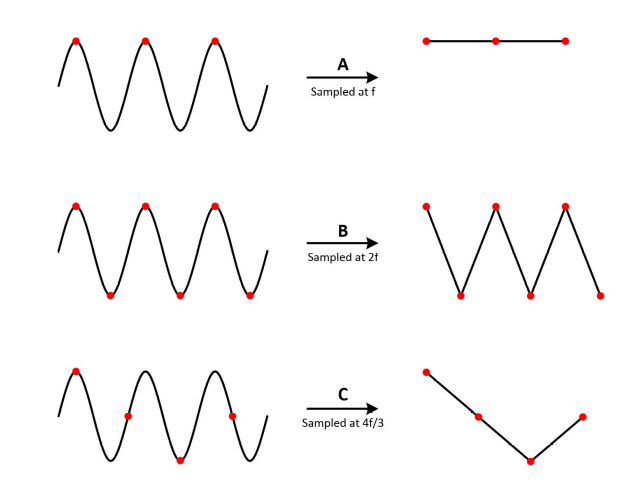
\includegraphics[width=0.6\textwidth]{Screenshot_20200224_121935.png}
    \caption{Minimale sample rate}
\end{figure}

\subsubsection{Aliasing}
= High Frequency signaal als Low Frequency 'spooksignaal' detecteren 
\begin{itemize}
    \item Treedt op bij onvoldoende hoge sample rate
    \item Anti-Aliasing filter (low-pass filter) beperkt signaal onder nyquist frequentie
\end{itemize}

\begin{figure}[H]
    \centering
    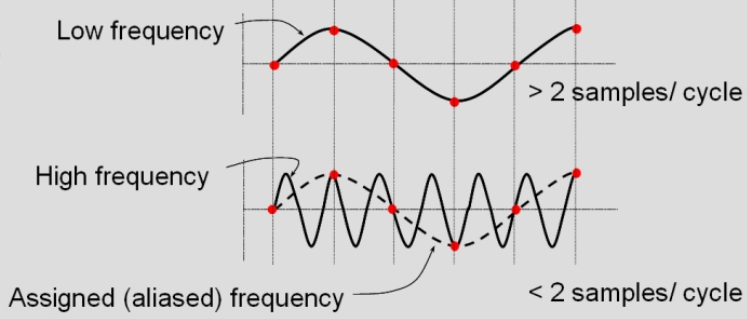
\includegraphics[width=0.7\textwidth]{Screenshot_20200224_122204.png}
    \caption{Anti-aliasing filter}
\end{figure}

\subsubsection{Oversampling}
\begin{itemize}
    \item Sampelen met veelvoud van nyquist frequentie
    \item Kan worden gebruikt om de resolutie op te voeren
    \item Kan worden gebruikt om digitaal (DSP) te filteren
    \item Verhoogt het effectieve aantal bits van de ADC
    \begin{itemize}
        \item \underline{Voorbeeld:} 20bit ADC met 256x OS = 24bit effectieve resolutie
    \end{itemize}
    \item Undersampling $\rightarrow$ specifiek gebruik bij mixers
\end{itemize}

\subsection{Implementatie en types}
\begin{itemize}
    \item De comparator
    \item Bekeken als 1-bit ADC
\end{itemize}

\begin{figure}[H]
    \centering
    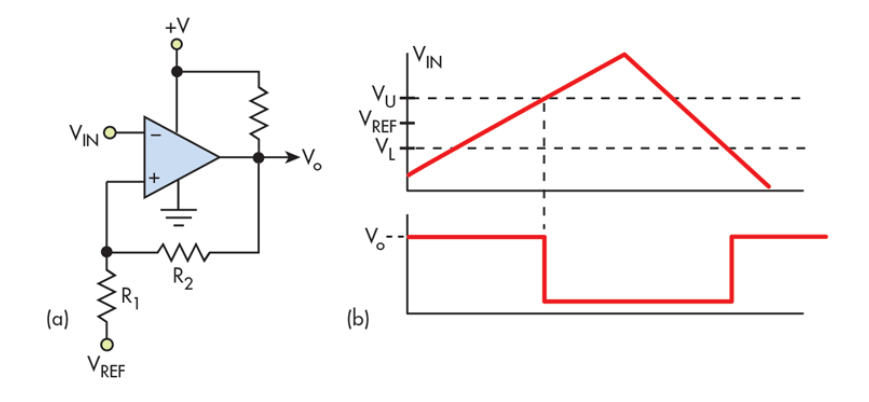
\includegraphics[width=0.7\textwidth]{Screenshot_20200224_122504.png}
    \caption{Comparator}
\end{figure}

\subsubsection{Flash ADC}
\begin{itemize}
    \item Comparator per 'level'
    \item Zeer snel = directe omzetting
    \item Complex \& High power
    \item Lagere resoluties
\end{itemize}

\begin{figure}[H]
    \centering
    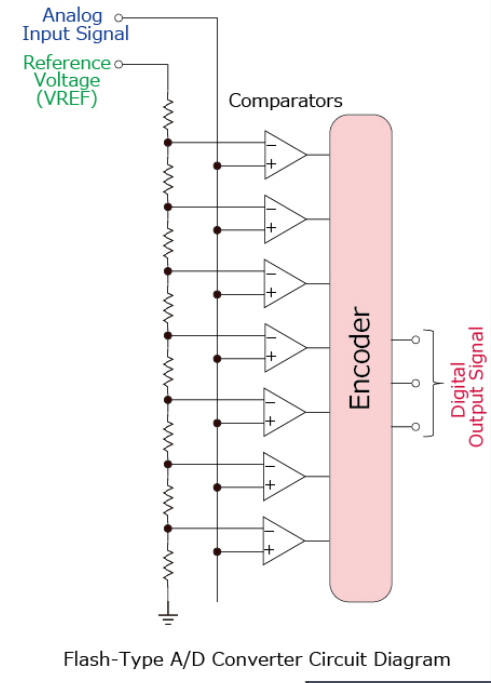
\includegraphics[width=0.5\textwidth]{Screenshot_20200224_122635.png}
    \caption{Flash ADC}
\end{figure}

\subsubsection{Successive approximation ADC}
\begin{itemize}
    \item Gebruikt 1 comparator
    \item Vergelijkt een opgewekte spanning met het signaal
    \item Hoge resolutie mogelijk
    \item Trager
    \item Relatief goedkoop
\end{itemize}

\begin{figure}[H]
    \centering
    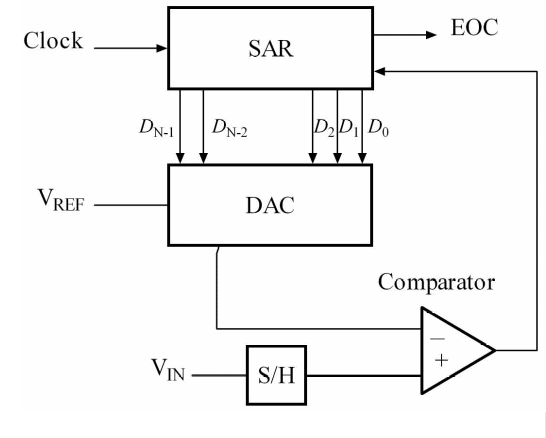
\includegraphics[width=0.7\textwidth]{Screenshot_20200224_122846.png}
    \caption{Successive approximation ADC}
\end{figure}

\section{Digitaal naar analoog conversie}
\begin{figure}[H]
    \centering
    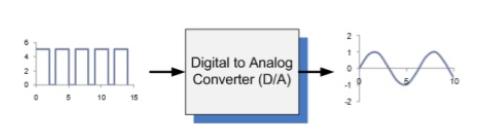
\includegraphics[width=0.7\textwidth]{Screenshot_20200224_115212.png}
    \caption{Digitaal naar analoog (DA converter)}
\end{figure}

\begin{itemize}
    \item Omzetten digitale naar analoge waarde
    \item Range
    \item Resolutie
    \item Samplefrequentie
\end{itemize}

\subsection{Simpele DAC}
\begin{itemize}
    \item Binair $\Rightarrow$ analoge waarde
    \item \underline{Voorbeeld}: weerstandsnetwerk
\end{itemize}

\begin{figure}[H]
    \centering
    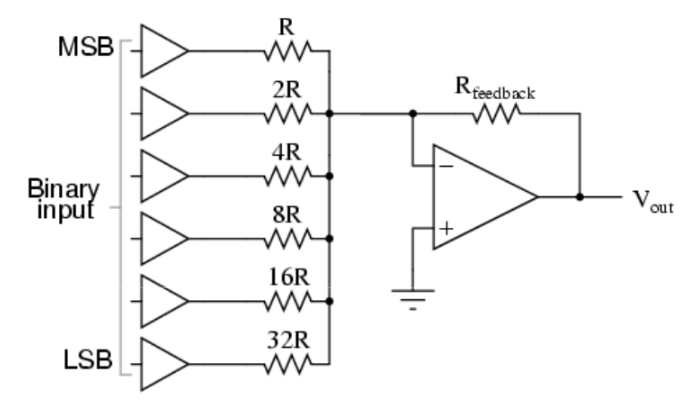
\includegraphics[width=0.7\textwidth]{Screenshot_20200224_123043.png}
    \caption{Weerstandsnetwerk}
\end{figure}

\subsection{Simpele DAC met PWM}
\begin{itemize}
    \item PWM == digitaal signaal
    \item Door variatie van duty-cycle kan de gemiddelde waarde worden gevarieerd
    \item Door filteren kan de blokgolf worden omgezet in een variabele analoge waarde 
\end{itemize}

\begin{figure}[H]
    \centering
    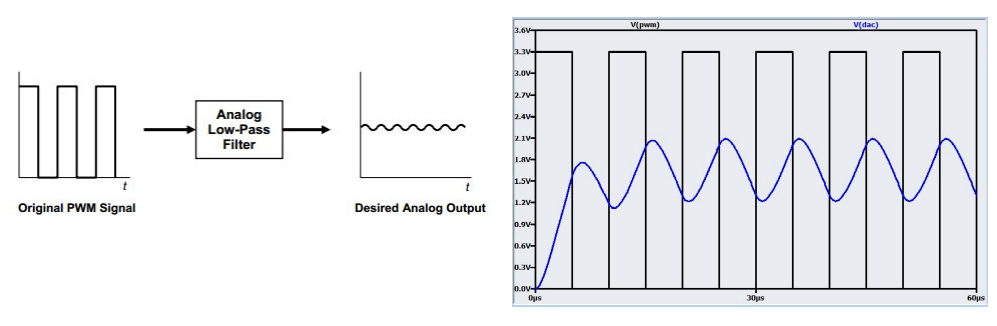
\includegraphics[width=0.7\textwidth]{Screenshot_20200224_123240.png}
    \caption{DAC met PWM}
\end{figure}

\subsection{Andere types}
\begin{itemize}
    \item $\Sigma\Delta$ (sigma delta) = herhaaldelijk downsampelen
    \item $I^2S$ DAC
    \item Nog zeer veel andere overwegingen:
    \begin{itemize}
        \item THD (Harmonische vervorming)
        \item Faseruis
        \item \dots
    \end{itemize}
\end{itemize}

\subsection{Extra info over AD/DA conversie:}
\begin{itemize}
    \item \url{https://en.wikipedia.org/wiki/Digital-to-analog_converter}
    \item \url{https://en.wikipedia.org/wiki/Analog-to-digital_converter}
    \item \url{https://en.wikipedia.org/wiki/Nyquist%E2%80%93Shannon_sampling_theorem}
    \item \url{https://en.wikipedia.org/wiki/Nyquist_rate}
    \item \url{https://en.wikipedia.org/wiki/Pulse-width_modulation}
    \item \url{https://en.wikipedia.org/wiki/Delta-sigma_modulation}
\end{itemize}

\section{Modulatie}
\begin{itemize}
    \item Informatie toevoegen aan een draaggolf
    \item Door de variatie van minstens een van de eigenschappen van deze draaggolf
\end{itemize}

\begin{figure}[H]
    \centering
    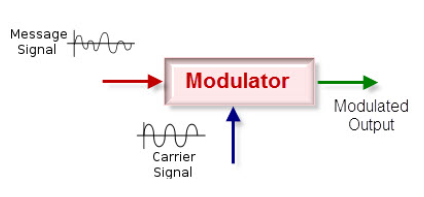
\includegraphics[width=0.9\textwidth]{Screenshot_20200302_115326.png}
    \caption{Modulatie}
\end{figure}

\subsection{Demodulatie}
= Het terugwinnen van de informatie uit de gemoduleerde draaggolf

\begin{figure}[H]
    \centering
    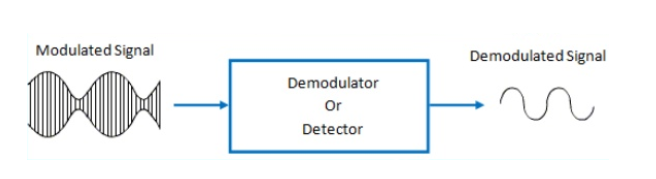
\includegraphics[width=0.9\textwidth]{Screenshot_20200302_115359.png}
    \caption{Demodulatie}
\end{figure}

\subsection{Modem}
= \bold{Mo}dulator + \bold{Dem}odulator

\begin{figure}[H]
    \centering
    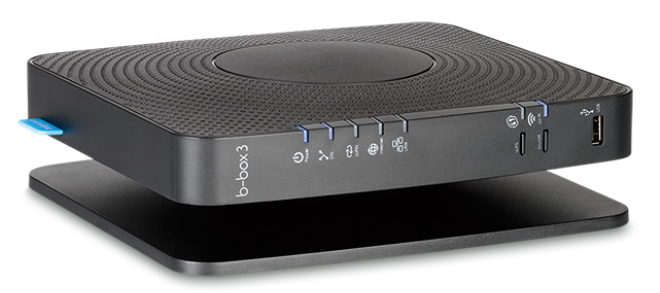
\includegraphics[width=0.6\textwidth]{Screenshot_20200302_115504.png}
    \caption{Modem}
\end{figure}

\subsection{Waarom?}

\begin{itemize}
    \item Interconnectie van IoT devices
    \item Vaak draadloos
\end{itemize}

\begin{figure}[H]
    \centering
    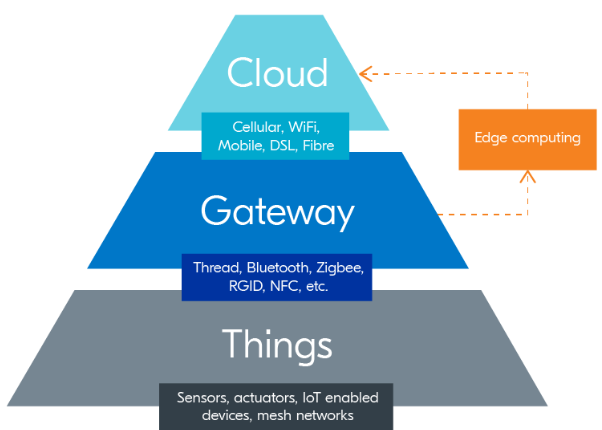
\includegraphics[width=0.6\textwidth]{Screenshot_20200302_115646.png}
    \caption{Interconnectie van devices}
\end{figure}

\subsection{Hoe?}
\begin{itemize}
    \item Draaggolf of carrier
    \item Signaal met een zekere (hogere) frequentie
\end{itemize}

\subsection{Draaggolf}
= carrier

\begin{figure}[H]
    \centering
    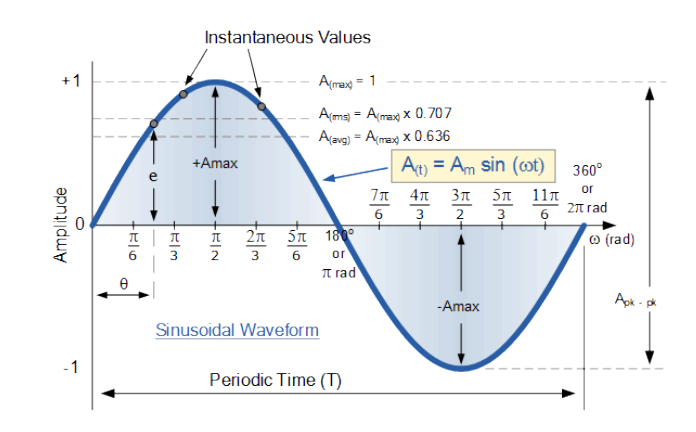
\includegraphics[width=0.8\textwidth]{Screenshot_20200302_115827.png}
    \caption{Draaggolf}
\end{figure}

\subsubsection{Parameters van een draaggolf}

\begin{itemize}
    \item Amplitude
    \item Frequentie / Periode
\end{itemize}

\subsection{Simpele modulatie}
\begin{itemize}
    \item Aan/uit schakelen van de draaggolf
    \item CW = continuous wave
    \item Bv: Morse code
\end{itemize}

\begin{figure}[H]
    \centering
    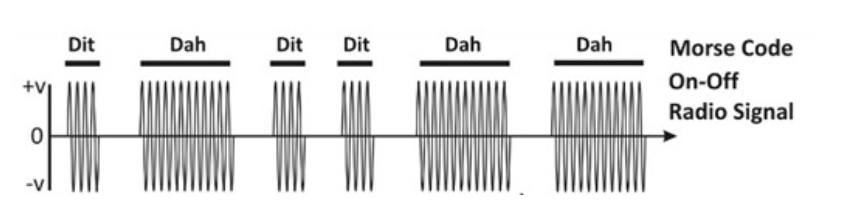
\includegraphics[width=0.8\textwidth]{Screenshot_20200302_120000.png}
    \caption{Morse code}
\end{figure}

\subsection{Amplitude modulatie (=AM)}
\begin{itemize}
    \item Aanpassen van de amplitude v/d draaggolf
\end{itemize}

\begin{figure}[H]
    \centering
    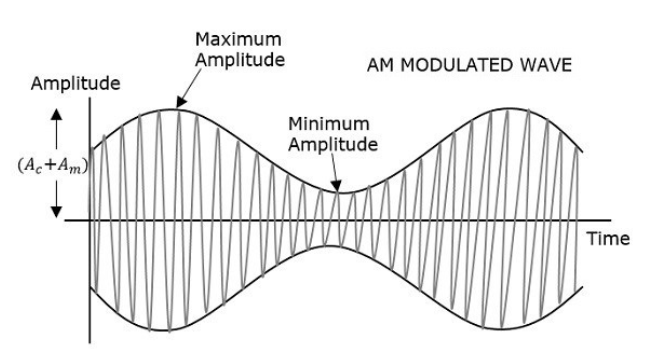
\includegraphics[width=0.8\textwidth]{Screenshot_20200302_120121.png}
    \caption{Amplitudemodulatie (1)}
\end{figure}

\begin{figure}[H]
    \centering
    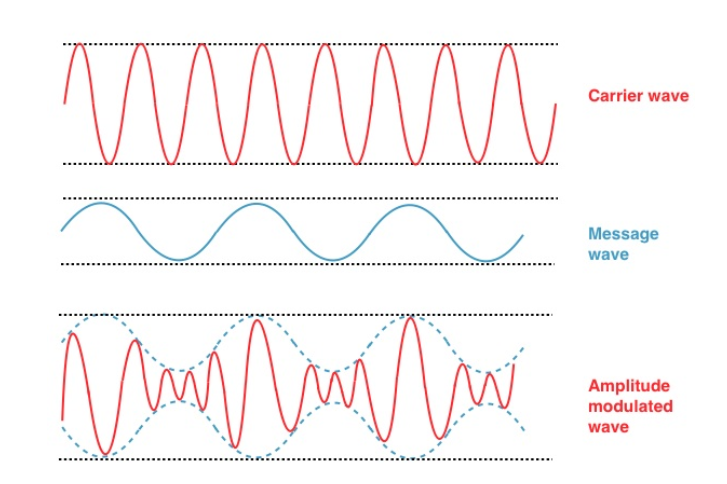
\includegraphics[width=0.8\textwidth]{Screenshot_20200302_120147.png}
    \caption{Amplitudemodulatie (2)}
\end{figure}

\begin{itemize}
    \item Radio LW/MW/SW AM
    \item Typisch gebruikt op 'lagere' HF banden: 100kHz - 60MHz
\end{itemize}

\subsubsection{Overmodulatie}
\begin{itemize}
    \item Modulatiediepte (modulatie index)
\end{itemize}

\begin{figure}[H]
    \centering
    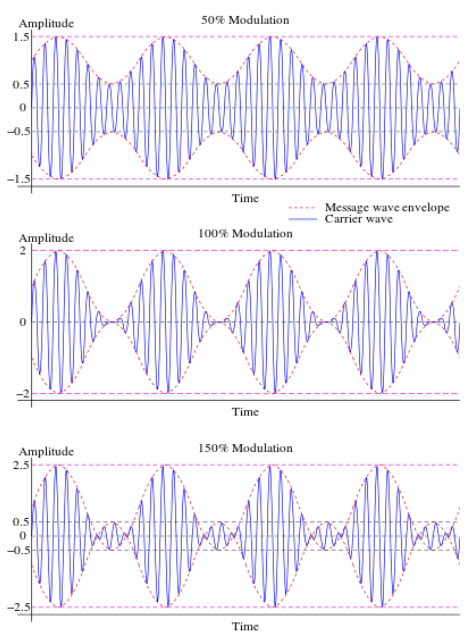
\includegraphics[width=0.8\textwidth]{Screenshot_20200302_120354.png}
    \caption{Overmodulatie}
\end{figure}

\subsubsection{AM bandbreedte}
\begin{itemize}
    \item Bandbreedte van een AM signaal:
    \begin{itemize}
        \item Centerfrequentie = draaggolffrequentie
        \item 2x frequentie van gemoduleerd signaal in totaal
    \end{itemize}
\end{itemize}

\begin{figure}[H]
    \centering
    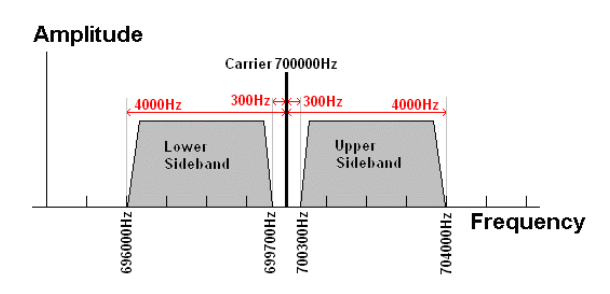
\includegraphics[width=0.8\textwidth]{Screenshot_20200302_120508.png}
    \caption{AM bandbreedte}
\end{figure}

\subsubsection{SSB modulatie (USB/LSB)}
\begin{itemize}
    \item Alle informatie zit in elke sideband (zijband) bij AM
    \item Carrier + 1 sideband wegfilteren = reductie van de bandbreedte
    \item Efficienter gebruik van het spectrum
    \item Moeilijk om goed te demoduleren
\end{itemize}
\begin{figure}[H]
    \centering
    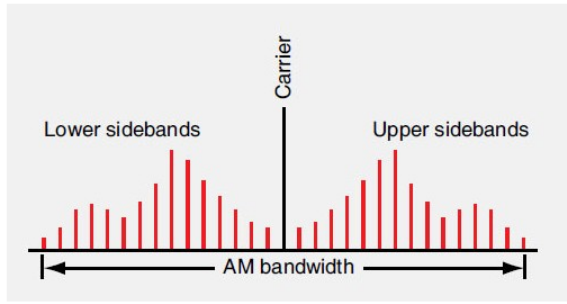
\includegraphics[width=0.7\textwidth]{Screenshot_20200315_153734.png}
    \caption{Zijbanden AM band}
\end{figure}

\begin{figure}[H]
    \centering
    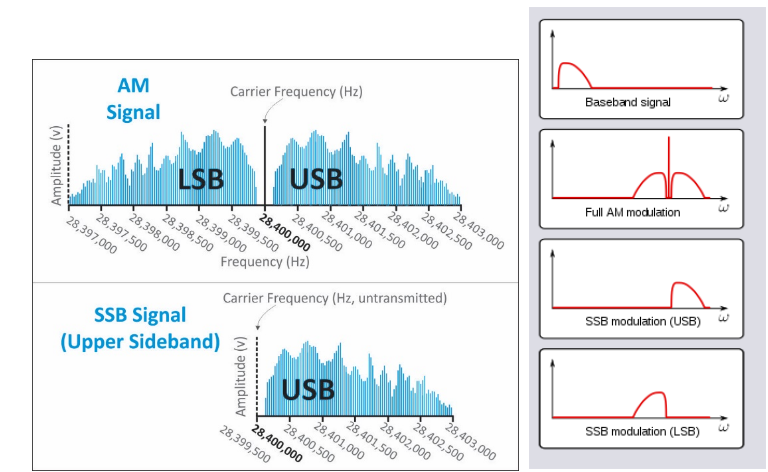
\includegraphics[width=\textwidth]{Screenshot_20200302_120812.png}    
    \caption{SSB Modulatie: we zenden alleen 1 van de zijbanden}
\end{figure}

\subsubsection{ASK Modulatie}
\begin{itemize}
    \item Amplitude shift keying
    \item Vorm van AM-modulatie voor digitale signalen
    \item Mogelijk met meerdere signaalniveaus
    \item 4-level ASK
\end{itemize}

\begin{figure}[H]
    \centering
    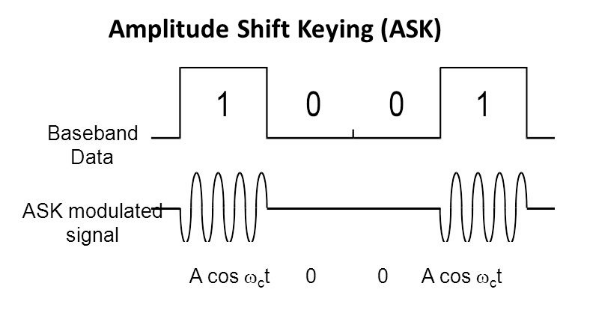
\includegraphics[width=0.6\textwidth]{Screenshot_20200302_121007.png}
    \caption{ASK}
\end{figure}

\begin{figure}[H]
    \centering
    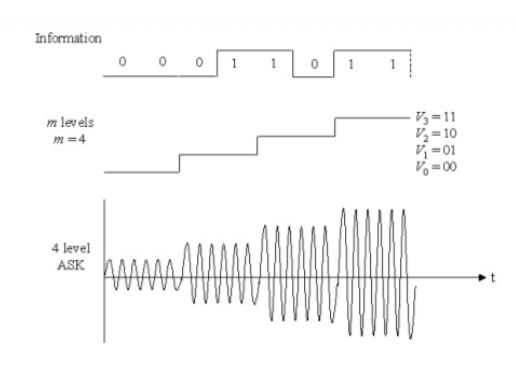
\includegraphics[width=0.6\textwidth]{Screenshot_20200302_121031.png}
    \caption{4 level ASK}
\end{figure}

\subsection{Frequentie modulatie (=FM)}
\begin{itemize}
    \item Variatie in de frequentie van de draaggolf
    \item FM radio 88MHz - 108MHz
    \item VHF Maritieme radio
    \item UHF PMR Radios
\end{itemize}

\begin{figure}[H]
    \centering
    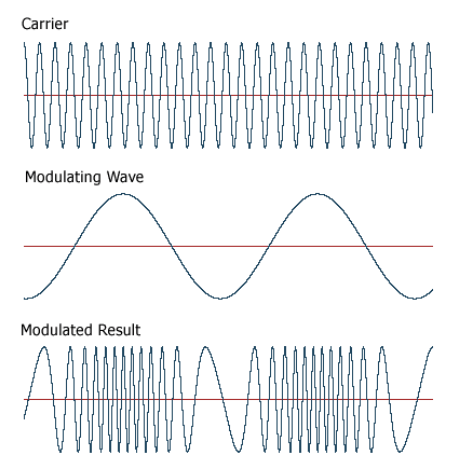
\includegraphics[width=0.6\textwidth]{Screenshot_20200302_121335.png}
    \caption{Frequentie modulatie}
\end{figure}

\subsubsection{FSK modulatie}
\begin{itemize}
    \item Frequency Shift Keying
    \item Vorm van FM
    \item Wisselen tussen 2 of meer frequenties
\end{itemize}

\begin{figure}[H]
    \centering
    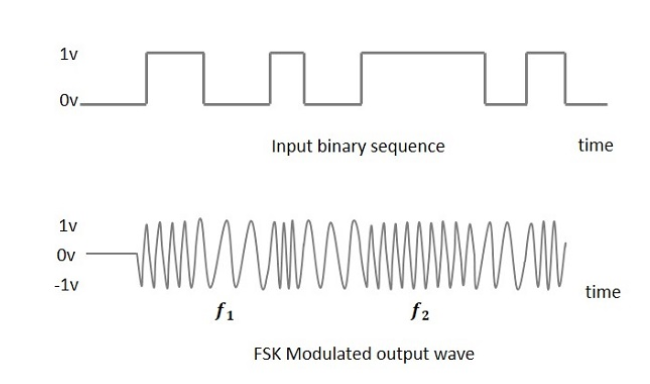
\includegraphics[width=0.6\textwidth]{Screenshot_20200302_121458.png}
    \caption{FSK}
\end{figure}

\subsubsection{FM Modulatie}
\begin{itemize}
    \item Carrier is altijd op 100\% amplitude aanwezig tijdens transmissie
    \item Minder ruis, betere kwaliteit voor audio dan AM
    \item Hogere bandbreedte $\Rightarrow$ Meer stroomverbruik
    \item WFM (Wide FM), NFM (Narrow FM), FM
\end{itemize}

\begin{figure}[H]
    \centering
    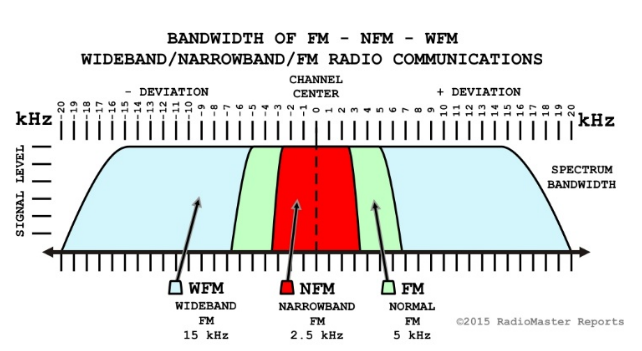
\includegraphics[width=0.8\textwidth]{Screenshot_20200302_121650.png}
    \caption{Bandbreedte FM - NFM - WFM}
\end{figure}

\subsubsection{Fase modulatie}
\begin{itemize}
    \item Faseverschuiving van een signaal
\end{itemize}

\begin{figure}[H]
    \centering
    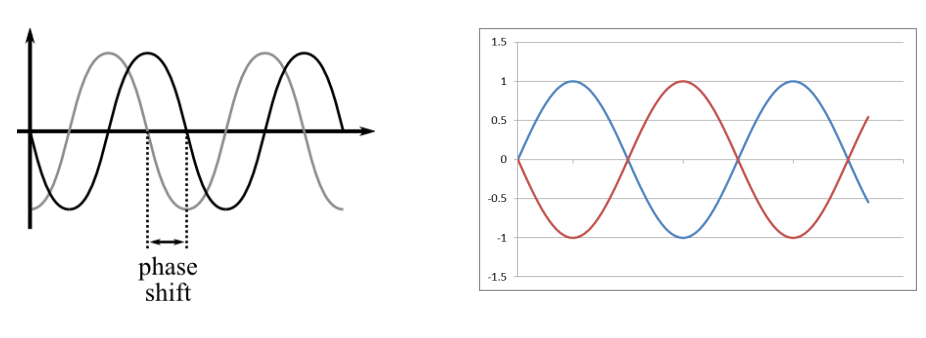
\includegraphics[width=0.8\textwidth]{Screenshot_20200302_121855.png}
    \caption{Faseverschuiving}
\end{figure}

\subsubsection{PSK modulatie}
\begin{itemize}
    \item Phase shift keying
    \item Bij wisselen van bit $\Rightarrow$ fase omkeren
\end{itemize}

\begin{figure}[H]
    \centering
    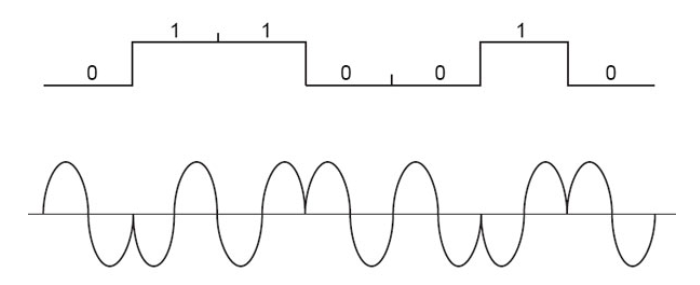
\includegraphics[width=0.6\textwidth]{Screenshot_20200302_122031.png}
    \caption{Fasemodulatie}
\end{figure}

\subsubsection{Phase Shift Modulatie}
\begin{itemize}
    \item BPSK $\Rightarrow$ Binary PSK = 2 fase
    \item QPSK $\Rightarrow$ Quadrature PSK = 4 fase
\end{itemize}

\begin{figure}[H]
    \centering
    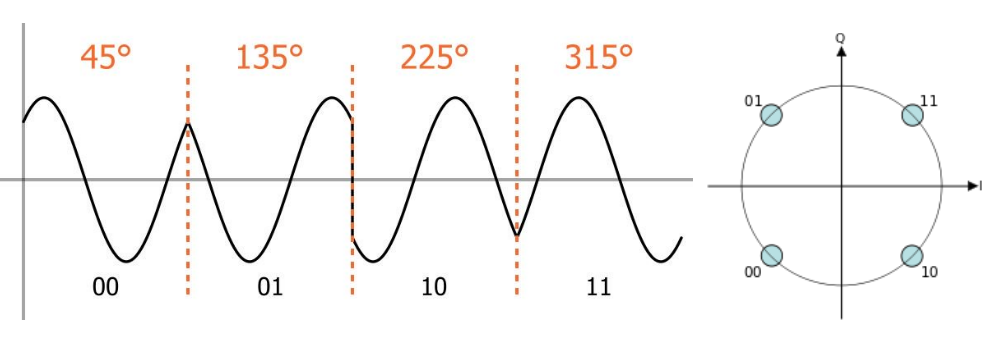
\includegraphics[width=0.6\textwidth]{Screenshot_20200302_122452.png}
    \caption{}
\end{figure}

\subsubsection{QAM modulatie}
\begin{itemize}
    \item Quadrature amplitude modulatie
    \item Informatie zit \dots
    \begin{itemize}
        \item de amplitude (zoals bij ASK)
        \item de fase (zoals bij PSK)
    \end{itemize}
    \item Meerdere symbolen
    \begin{itemize}
        \item 4-QAM
        \item 16-QAM
        \item 64-QAM
        \item \dots
    \end{itemize}
\end{itemize}

\begin{figure}[H]
    \centering
    \includegraphics[width=0.3\textwidth]{Screenshot_20200315_160021.png}
    \caption{QAM modulatie}
\end{figure}


\begin{itemize}
    \item DAB+ $\Rightarrow$ 4/16/64 - QAM
    \item Hogere transmissiesnelheid
    \item Gevoeliger voor fouten
\end{itemize}

\begin{figure}[H]
    \centering
    \includegraphics[width=0.6\textwidth]{Screenshot_20200302_123030.png}
    \caption{16-, 64-, 256-QAM}
\end{figure}

\subsubsection{Bandbreedte / vermogen}
\begin{itemize}
    \item Meer bandbreedte = hogere snelheid
    \item Meer bandbreedte = hoger vermogen nodig
\end{itemize}

\begin{figure}[H]
    \centering
    \includegraphics[width=0.6\textwidth]{Screenshot_20200302_122703.png}
    \caption{}
\end{figure}


\subsubsection{Waarom Narrow-band?}
\begin{itemize}
    \item Oppervlakte van het signaal = Power
    \item Bij smalbandige signalen $\Rightarrow$ betere SNR (signaal-naar-ruis) verhouding bij hetzelfde vermogen
    \item Om met een klein vermogen heel grote afstanden overbruggen
    \item Zeer traag
\end{itemize}

\begin{figure}[H]
    \centering
    \includegraphics[width=0.6\textwidth]{Screenshot_20200302_123310.png}
    \caption{Waarom Narrow-band: narrow-band kan makkelijker boven ruisniveau}
\end{figure}

\begin{figure}[H]
    \centering
    \includegraphics[width=0.8\textwidth]{Screenshot_20200302_122906.png}
    \caption{Voorbeeld: NB-IoT}
\end{figure}

\begin{figure}[H]
    \centering
    \includegraphics[width=0.4\textwidth]{Screenshot_20200302_122954.png}
    \caption{Voorbeeld: Telefoonmodem (\url{https://www.youtube.com/watch?v=ckc6XSSh52w})}
\end{figure}

\section{RF-spectrum}

\begin{figure}[H]
    \centering
    \includegraphics[width=\textwidth]{Screenshot_20200309_115132.png}
    \caption{Radiogolven op het spectrum}
\end{figure}

\subsection{Beschikbare bandbreedte}
\begin{itemize}
    \item In de hogere frequentiebanden is meer bandbreedte beschikbaar
    \item Voorbeeld:
    \begin{itemize}
        \item 2.4GHz WiFi: 20MHz bandbreedte
        \item 5GHZ 802.11ac WiFi: 80MHz bandbreedte
        \item 1 WiFi kanaal > volledige AM-radio LW + MW + SW band
    \end{itemize}
    \item Meer bandbreedte = mogelijk hogere datarates
\end{itemize}

\begin{figure}[H]
    \centering
    \includegraphics[width=0.4\textwidth]{Screenshot_20200315_160828.png}
    \caption{Impact van hogere bandbreedtes op datarates}
\end{figure}

\subsection{Licenties en licentievrije banden}
\begin{itemize}
    \item Beheer van het spectrum 
    \item In Belgie door het BIPT
    \item In de VS door het FCC
    \item Harmonisatie in Europa / VS / Azië
    \item \url{https://www.bipt.be/nl/operatoren/radio/frequentiebeheer/frequentieplan/tabel}
\end{itemize}

\subsection{ISM banden}
\begin{itemize}
    \item = Industrial / Scientific / Medical - Band
    \item Geen vergunning nodig voor gebruik
    \item Is aan strikte voorwaarden verbonden
    \begin{itemize}
        \item Maximaal vermogen
        \item Maximale transimissietijd
        \item Maximale periodiciteit van transmissies
        \item Maximale bandbreedte
        \item \dots
    \end{itemize}
    \item Specifieke banden zijn hiervoor vrijgegeven
\end{itemize}

\subsection{Interferentie}

\subsubsection{Co-channel interferentie}
Wat als meerdere systemen dezelfde band gebruiken?

\begin{figure}[H]
    \centering
    \includegraphics[width=\textwidth]{Screenshot_20200309_115759.png}
    \caption{Co-channel Interferentie}
\end{figure}

\subsubsection{Signaalseparatie}

\begin{itemize}
    \item Minimaal verschil is afhankelijk van modulatietype
    \item Voorbeeld:
    \begin{itemize}
        \item BPSK $>$ 10dB
        \item 256-QAM $>$ 40dB
    \end{itemize}
\end{itemize}

\begin{figure}[H]
    \centering
    \includegraphics[width=0.7\textwidth]{Screenshot_20200309_120012.png}
    \caption{Signaalseparatie}
\end{figure}

\subsubsection{Interferentie van naburige kanalen}
\begin{figure}[H]
    \centering
    \includegraphics[width=0.9\textwidth]{Screenshot_20200309_120313.png}
    \caption{Interferentie van naburige kanalen}
\end{figure}

\subsubsection{Interferentie van andere toestellen}
\begin{itemize}
    \item Ruis / atmosferische storingen
    \item SNR $\Rightarrow$ Signaal / Ruis verhouding
\end{itemize}

\begin{figure}[H]
    \centering
    \includegraphics[width=0.9\textwidth]{Screenshot_20200309_120624.png}
    \caption{Interferentie van andere toestellen}
\end{figure}

\subsection{Meten van interferentie}
\begin{itemize}
    \item Meten van WiFi kanalen kan met software 
    \item Software is niet in staat niet-WiFi signalen te meten
    \item Kan worden gemeten met een spectrum analyzer
\end{itemize}

\begin{figure}[H]
    \centering
    \includegraphics[width=0.6\textwidth]{Screenshot_20200309_120748.png}
    \caption{Meten van interferentie}
\end{figure}

\subsection{Golflengte}
\begin{itemize}
    \item Golflengte in meter is een andere wijze om de frequentie weer te geven
    \item Relevant bij antennes en transmissielijnen
    \item $\lambda = \frac{c}{f}$
    \item $c=$ lichtsnelheid = $299\ 792\ 458 \text{ m/s}$ 
\end{itemize}

\begin{figure}[H]
    \centering
    \includegraphics[width=0.6\textwidth]{Screenshot_20200309_121003.png}
    \caption{Golflengte $\lambda$}
\end{figure}

\subsubsection{Rekenvoorbeeld}
Frequentie van $102.1\text{ MHz}$
\begin{itemize}
    \item $\lambda = \frac{299\ 792\ 458 \text{ m/s}}{102.1\text{ MHz}} = 2.936\dots \text{ m}$
\end{itemize}
"De 70 cm band":
\begin{itemize}
    \item $f = \frac{(299\ 792\ 458)}{\lambda} = \frac{(299\ 792\ 458)}{0.7\ \text{m}} =  428\ 274\ 940\ \text{Hz} = 430\ \text{MHz}$
\end{itemize}

\subsection{Antennesysteem}
\begin{itemize}
    \item Een antenne stuurt / ontvangt zoveel mogelijk van de RF-energie op de gewenste frequentie
    \item $\Rightarrow$ resonantie van het antennesysteem op de gewenste frequentie
    \item Formaat van de antenne is vaak beperkende factor 
\end{itemize}

\begin{figure}[H]
    \centering
    \includegraphics[width=0.4\textwidth]{Screenshot_20200309_122045.png}
    \caption{}
\end{figure}

\subsubsection{De dipool antenne}
\begin{itemize}
    \item Zeer eenvoudig
    \item $\frac12 \lambda$ groot
    \item Vaak toegepast
    \item Kan worden 'opgeplooid'
\end{itemize}

\begin{figure}[H]
    \centering
    \includegraphics[width=0.8\textwidth]{Screenshot_20200309_122306.png}
    \caption{Dipool antenne}
\end{figure}

\subsubsection{Polarisatie van antennes}
\begin{figure}[H]
    \centering
    \includegraphics[width=\textwidth]{Screenshot_20200309_122403.png}
    \caption{Polarisatie van antennes}
\end{figure}

\subsubsection{Directionaliteit van antennes}
\begin{itemize}
    \item Omnidirectionele antenne
    \begin{itemize}
        \item Meestal dipolen of end-fed (=stukje draad)
        \item Discone
    \end{itemize}
    \item Directionele antenne (beam)
    \begin{itemize}
        \item Schotelantenne
        \item Yagi
        \item Patch
    \end{itemize}
\end{itemize}

\begin{figure}[H]
    \centering
    \includegraphics[width=\textwidth]{Screenshot_20200309_122609.png}
    \caption{Directionaliteit van antennes}
\end{figure}

\subsubsection{Stralingspatroon van antennes}
\begin{itemize}
    \item Gevoeligheid van antennes is niet overal hetzelfde
    \item Zeer afhankelijk van constructie en type antenne
\end{itemize}

\begin{figure}[H]
    \centering
    \includegraphics[width=\textwidth]{Screenshot_20200309_122734.png}
    \caption{Stralingspatroon van antennes}
\end{figure}

\subsubsection{Gain van een antenne}
\begin{itemize}
    \item Gain = versterking
    \item Uitgedrukt in dB
    \item Nooit 'magisch', er is altijd een trade-off
    \begin{itemize}
        \item Directionaliteit
        \item Bandbreedte
    \end{itemize}
\end{itemize}

\begin{figure}[H]
    \centering
    \includegraphics[width=\textwidth]{Screenshot_20200309_122914.png}
    \caption{Gain van een antenne}
\end{figure}

\subsection{Propagatie van RF-signalen}
\begin{itemize}
    \item Absorptie
    \item Reflectie
    \item Scattering
    \item Refractie
    \item Path loss
    \item \dots
\end{itemize}

\begin{figure}[H]
    \centering
    \includegraphics[width=0.6\textwidth]{Screenshot_20200309_123000.png}
    \caption{Propagatie van RF-signalen}
\end{figure}

\subsubsection{Path loss}
\begin{itemize}
    \item Verzwakking van het signaal met afstand zonder obstakels $\Rightarrow$ \underline{free space path loss}
    \item \bold{Oorzaak} uitdeinen van het signaal
    \item Verzwakking is exponentieel met de afstand
    \item Enkel afhankelijk van frequentie en afstand
    \item Hogere frequenties hebben hoger path loss
\end{itemize}

FSPL (dB) $= 20\cdot log_{10}(d) + 20\cdot log_{10}(f) + 32.44$
\begin{itemize}
    \item d = afstand in km
    \item f = frequentie in MHz
\end{itemize}

\subsubsection{Signaalverzwakking / path loss}
\begin{itemize}
    \item Meer verzwakking bij hogere frequenties
    \item Minder bandbreedte bij lagere frequenties
    \item Wat is beter?
    \begin{itemize}
        \item 2.4GHz WiFi
        \item 5GHz WiFi
    \end{itemize}
\end{itemize}

\begin{figure}[H]
    \centering
    \includegraphics[width=0.5\textwidth]{Screenshot_20200309_123426.png}
    \caption{Signaalverzwakking / path loss}
\end{figure}

\subsubsection{Dynamic Rate Shifting (DRS)}
\begin{itemize}
    \item Modulatietechniek dynamisch aanpassen aan de signaalcondities
    \item Minder gunstige SNR $\Rightarrow$ Lagere datarate kiezen
    \item Andere modulatievorm 
\end{itemize}

\begin{figure}[H]
    \centering
    \includegraphics[width=0.7\textwidth]{Screenshot_20200309_123624.png}
    \caption{Dynamic Rate Shifting}
\end{figure}

\subsubsection{Reflectie}
\begin{itemize}
    \item Signaal wordt gereflecteerd
    \item Bv:
    \begin{itemize}
        \item Door metalen objecten
        \item Water
        \item \dots
    \end{itemize}
\end{itemize}

\begin{figure}[H]
    \centering
    \includegraphics[width=0.7\textwidth]{Screenshot_20200309_124220.png}
    \caption{Reflectie}
\end{figure}

\subsubsection{Absorptie}

\begin{itemize}
    \item Signaal kan deels of volledig worden geabsorbeerd 
    \item Resulteert in verzwakking van bruikbare signaal
    \item Verzwakking = attentuatie typisch in dB
\end{itemize}

\begin{figure}[H]
    \centering
    \includegraphics[width=0.7\textwidth]{Screenshot_20200309_124354.png}
    \caption{Absorptie}
\end{figure}

\subsubsection{Doordringbaarheid}
\begin{itemize}
    \item Hogere frequenties worden gemakkelijk tegengehouden door objecten
    \item Lagere frequenties kunnen gemakkelijker door objecten heen
\end{itemize}

\begin{figure}[H]
    \centering
    \includegraphics[width=0.7\textwidth]{Screenshot_20200309_124451.png}
    \caption{Doordringbaarheid}
\end{figure}

\subsubsection{Scattering}
\begin{itemize}
    \item Signaal wordt gereflecteerd in diverse richtingen
    \item Oneffen oppervlaktes
    \item Wolken materiaal bv zand, \dots
\end{itemize}

\begin{figure}[H]
    \centering
    \includegraphics[width=0.7\textwidth]{Screenshot_20200309_124533.png}
    \caption{Scattering}
\end{figure}

\subsubsection{Refractie}
\begin{itemize}
    \item Bij 2 media met verschillende dichtheid
    \item Afbuiging van het signaal
\end{itemize}

\begin{figure}[H]
    \centering
    \includegraphics[width=0.5\textwidth]{Screenshot_20200309_124610.png}
    \caption{Refractie}
\end{figure}

\subsubsection{Difractie}
\begin{itemize}
    \item RF-signaal wordt beïnvloed door obstakels
    \item Gaat er niet door maar “rond”, zoals water rond een paaltje in een rivier
    \item Verstoort / verminkt het RF-signaal
\end{itemize}

\begin{figure}[H]
    \centering
    \includegraphics[width=0.5\textwidth]{Screenshot_20200309_124659.png}
    \caption{Difractie}
\end{figure}

\subsubsection{Fresnel zones}
\begin{itemize}
    \item Golfmodel RF-signalen 
    \item Worden ook beïnvloed door objecten in nabijheid
    \item Niet enkel door objecten in line-of-sight
\end{itemize}

\begin{figure}[H]
    \centering
    \includegraphics[width=0.5\textwidth]{Screenshot_20200309_124752.png}
    \caption{Fresnel zones}
\end{figure}

\begin{itemize}
    \item Afhankelijk van frequentie en afstand
\end{itemize}

\begin{figure}[H]
    \centering
    \includegraphics[width=0.5\textwidth]{Screenshot_20200309_124825.png}
    \caption{Fresnel zone radius is afhankelijk van frequentie en afstand}
\end{figure}

\begin{itemize}
    \item Communiatie kan verstoord worden, zelfs door een object buiten de line-of-sight
\end{itemize}

\begin{figure}[H]
    \centering
    \includegraphics[width=0.5\textwidth]{Screenshot_20200309_125331.png}
    \caption{Verstoring door object in line-of-sight van transmissie}
\end{figure}

\subsubsection{Propagatie van RF-signalen}

\begin{itemize}
    \item Bepaalde effecten kunnen worden gebruikt
    \item Bv: Communicatie mbv reflectie op de ionosfeer
\end{itemize}

\begin{figure}[H]
    \centering
    \includegraphics[width=0.5\textwidth]{Screenshot_20200309_125500.png}
    \caption{communicatie mbv reflectie op de ionosfeer}
\end{figure}

\subsubsection{MIMO}

\begin{itemize}
    \item = Multiple In / Multiple Out
    \item Reflectie en scattering kan positief worden gebruikt 
    \item Beamforming
    \item Extra processing nodig
\end{itemize}

\begin{figure}[H]
    \centering
    \includegraphics[width=0.5\textwidth]{Screenshot_20200309_125719.png}
    \caption{MIMO}
\end{figure}

\subsubsection{Multiplexing}

\section{Seriele communicatie}
\subsection{Serieel vs parallel}

\begin{figure}[H]
    \centering
    \includegraphics[width=0.4\textwidth]{Screenshot_20200323_114507.png}
    \caption{Serieel vs parallel}
\end{figure}

\subsection{Parallelle communicatie}
\begin{itemize}
    \item Eenvoudig
    \item Sneller (bij eenzelfde kloksnelheid)
    \item Veel connecties
    \item Clock skew / jitter
\end{itemize}

\begin{figure}[H]
    \centering
    \includegraphics[width=0.5\textwidth]{Screenshot_20200323_114732.png}
    \caption{Parallelle communicatie}
\end{figure}

\subsubsection{Clock skew}
\begin{itemize}
    \item Verschillende vertraging tussen signalen
    \item Begrensd maximale klokfrequentie
\end{itemize}

\begin{figure}[H]
    \centering
    \includegraphics[width=0.4\textwidth]{Screenshot_20200323_114937.png}
    \caption{Clock skew}
\end{figure}

\subsection{Seriele communicatie}
\begin{itemize}
    \item Minder bekabeling
    \item Minder problemen met timing
    \item Minder last van crosstalk
    \item Complexer / SERDIS
\end{itemize}

\begin{figure}[H]
    \centering
    \includegraphics[width=0.4\textwidth]{Screenshot_20200323_115035.png}
    \caption{}
\end{figure}

\subsection{Serieel vs Parallel: wanneer gebruiken?}
\begin{itemize}
    \item Lange afstanden: serieel, want minder verbindingen
    \item Vroeger: lokale korte verbindingen, parallel
    \item Tegenwoordig: snelle lokale verbindingen, serieel
    \item ATA in harde schijven vervangen door SATA (Serial ATA)
    \item PCI vervangen door PCI Express op moederborden, ook serieel
\end{itemize}

\subsection{SERDIS}
\begin{itemize}
    \item Serialiser
    \item Deserialiser
\end{itemize}

\begin{figure}[H]
    \centering
    \includegraphics[width=0.4\textwidth]{Screenshot_20200323_115743.png}
    \caption{SERDIS}
\end{figure}

\subsubsection{Implementatie}
Met schuifregister
\begin{itemize}
    \item SIPO (serial in parallel out)
    \item PISO (parallel in serial out)
\end{itemize}

\begin{figure}[H]
    \centering
    \includegraphics[width=0.7\textwidth]{Screenshot_20200323_115735.png}
    \caption{Schuifregister}
\end{figure}

\subsection{Duplex}
\begin{itemize}
    \item Full-duplex
    \item Half-duplex
    \item Simplex
\end{itemize}

\begin{figure}[H]
    \centering
    \includegraphics[width=0.7\textwidth]{Screenshot_20200323_115925.png}
    \caption{Verschillende verbindingen}
\end{figure}

\begin{figure}[H]
    \centering
    \includegraphics[width=0.7\textwidth]{Screenshot_20200323_120141.png}
    \caption{Full duplex}
\end{figure}

\subsection{Flow Control}
Beperken hoeveel de zender kan/mag versturen.

\begin{itemize}
    \item Kan in hardware $\Rightarrow$ extra verbindingen
    \item Kan in software $\Rightarrow$ controle karakters
\end{itemize}

\begin{itemize}
    \item Hardware (CTS / RTS / Enable / \dots)
    \item Xon / Xoff: starten/stoppen van het signaal
    \item No
\end{itemize}

\subsection{Synchroon vs Asynchroon}
\begin{itemize}
    \item Synchroon $\Rightarrow$ Gebruikt een aparte kloklijn
    \item Asynchroon $\Rightarrow$ Geen kloklijn
\end{itemize}

\begin{figure}[H]
    \centering
    \includegraphics[width=0.7\textwidth]{Screenshot_20200323_120525.png}
    \caption{Kloklijn}
\end{figure}

\subsection{Synchrone seriele communicatie}
\begin{itemize}
    \item 1 device genereert de klok
    \item Alle transmissies synchroniseren op deze klok
    \item Kan op de stijgende flank of op de dalende flank 
\end{itemize}

\begin{figure}[H]
    \centering
    \includegraphics[width=0.4\textwidth]{Screenshot_20200323_120955.png}
    \caption{Synchrone seriele communicatie}
\end{figure}


\subsection{Asynchrone seriele communicatie}
\begin{itemize}
    \item Werkt zonder aparte kloklijn
    \item Dus minder verbindingen
    \item Syncrhonisatie door ontvanger noodzakelijk
    \item Start en stop bit (/conditie) noodzakelijk
\end{itemize}


\begin{figure}[H]
    \centering
    \includegraphics[width=0.7\textwidth]{Screenshot_20200323_121104.png}
    \caption{Asynchrone seriele communicatie}
\end{figure}

\subsubsection{Parameters}
\begin{itemize}
    \item Baudrate (=bits per seconde)
    \item Aantal databits
    \item Pariteitsbit
    \item Aantal stop bits
\end{itemize}

\subsubsection{Standaarnotering}
\begin{itemize}
    \item Bijvoorbeeld: 9600-8-N-1
    \item Baudrate = 9600
    \item 8 = aantal databits
    \item N = welke pariteit
    \item 1 = aantal stop-bits
\end{itemize}

\subsubsection{Baudrate}
= Snelheid in bits/seconde
\begin{itemize}
    \item Niet alle bits zijn databits
    \item Start, stop en pariteitsbit transporteren geen data
\end{itemize}

\bold{Bijvoorbeeld}
\begin{itemize}
    \item 8-N-1 $\Rightarrow$ 80\% efficientie
    \item 8 databits van in totaal $8+1+1=10\ \text{bits} = 8/10\ \text{of}\ 80\%$
\end{itemize}

\subsubsection{Aantal databits}
\begin{itemize}
    \item Typisch 7 of 8 databits
    \item 7 bit is voldoende voor niet extended ASCII
    \item 8 bit $\Rightarrow$ noodzakelijk voor binaire transmissie (bv voor firmware)
    \item XMODEM / ZMODEM protocollen voor binaire transfers (weinig gebruikt want er bestaan nieuwere protocollen zoals USP)
\end{itemize}

\subsubsection{Pariteit}
= Foutdetectie
\\
\bold{Soorten pariteit}
\begin{itemize}
    \item Even (E)
    \item Odd (O)
    \item None (N)
\end{itemize}

Aantal 1 bits tellen en dit aantal steeds even of oneven maken

\subsubsection{Stopbits}
\begin{itemize}
    \item Aantal bits op het einde van een data-bit reeks
    \item $1/1.5/2\ $ bits
\end{itemize}

\subsection{Snelheid}
\begin{itemize}
    \item 1 transmissie = 1 karakter
    \item Aantal bits voor 1 karakter = som alle bits
    \item Baudrate in bits/seconde
\end{itemize}

\bold{Voorbeeldoefening}
\begin{itemize}
    \item 300-8-E2
    \item 8 databits + 1 pariteit + 2 stopbits + 1 startbit = 12bits
    \item 300 bits/seconde = 300 / 12 = 25 CPS (=characters per second)
\end{itemize}

\subsection{Meerdere deelnemers}
\begin{itemize}
    \item Multi device bus
    \item Daisy chain (=de ene deelnemer hangt aan de andere tot we aan de laatste deelnemer hangen, dan hangt de laatste ook aan de eerste)
    \item $\Rightarrow$ afspraken/arbitrage is noodzakelijk
\end{itemize}


\begin{figure}[H]
    \centering
    \includegraphics[width=0.7\textwidth]{Screenshot_20200323_122755.png}
    \caption{Meerdere deelnemers op een bus}
\end{figure}

\subsection{Manchester encoding}
\begin{itemize}
    \item Manier om asynchroon te werken, maar de klok en datasignaal in 1 signaal te stoppen
    \item Altijd voldoende omschakeling (bv voor RF tranmissie)
    \item Met AND-operatie
\end{itemize}

\begin{figure}[H]
    \centering
    \includegraphics[width=0.9\textwidth]{Screenshot_20200323_123031.png}
    \caption{Manchester encoding: Clock \& Data = OUTPUT}
\end{figure}

\subsection{Differentiele communicatie}
\begin{itemize}
    \item Differential vs single-ended
    \item Zowel synchroon als asynchroon kan differentieel of single-ended werken
    \item Minder gevoelig aan storingen
\end{itemize}


\begin{figure}[H]
    \centering
    \includegraphics[width=0.7\textwidth]{Screenshot_20200323_123305.png}
    \caption{Single-ended (boven) vs Differentieel (onder)}
\end{figure}

\begin{figure}[H]
    \centering
    \includegraphics[width=0.7\textwidth]{Screenshot_20200323_123231.png}
    \caption{Wat er gebeurt bij storing bij een differentieel signaal}
\end{figure}

\subsection{Benoeming van signalen}
Deze namen vind je vaak op protocollen en devices zoals de Arduino, RPi, \dots

\begin{itemize}
    \item RX $\Rightarrow$ receiver
    \item TX $\Rightarrow$ transmitter
    \item Dit is mogelijks ambigu zijn. Oplossing: nieuwe naamgeving:
    \begin{itemize}
        \item MOSI $\Rightarrow$ Master Out Slave In
        \item MISO $\Rightarrow$ Master In Slave Out
    \end{itemize}
    \item CS $\Rightarrow$ Chip Select
    \item EN $\Rightarrow$ Enable
    \item R/W $\Rightarrow$ Read/Write
    \item SCL $\Rightarrow$ Serial Clock
    \item SDA $\Rightarrow$ Serial Data
    \item Minder gebruikte signalen (Niet expliciet te kennen)
    \begin{itemize}
        \item CTS 
        \item DTR
    \end{itemize}
    \item \dots
\end{itemize}

\subsection{Protocollen}
= Standaarden voor communicatieafspraken

\begin{figure}[H]
    \centering
    \includegraphics[width=0.7\textwidth]{Screenshot_20200323_124324.png}
    \caption{Schema dat toont hoe het protocol werkt}
\end{figure}

\end{document}
